\documentclass[12pt,a4paper,oneside,article]{memoir}

\usepackage{polyglossia}
\setdefaultlanguage{english}
\usepackage{fontspec}

\defaultfontfeatures{Ligatures=TeX,Scale=MatchLowercase,Renderer=OpenType}
\defaultfontfeatures[\rmfamily]{Scale = 1}
\newfontfeature{Microtype}{protrusion=default;expansion=default;}
\usepackage[final]{microtype}
\usepackage{mathtools,amssymb}
\usepackage{unicode-math}

\setmainfont[Microtype,Microtype,Ligatures={Common,TeX},Numbers=OldStyle]{TeX Gyre Pagella}
\setsansfont[Microtype,Numbers=OldStyle]{TeX Gyre Heros}
\setmonofont{TeX Gyre Cursor}
\setmathfont{TeX Gyre Pagella Math}

\usepackage{subfiles}
\usepackage{tabulary}
\usepackage{booktabs}
\usepackage{multirow}
\usepackage{float}
\usepackage{amsmath,amsfonts,amssymb}
\usepackage{mathtools}
\usepackage[shortlabels]{enumitem}
\usepackage{subcaption}

\usepackage{tikz}
\usepackage{graphicx}
\usepackage{hyperref}
\hypersetup{hidelinks}
% \hypersetup{colorlinks = true}
\usepackage{xcolor, colortbl, array}

\usepackage{titling}
\usepackage{listings}
\lstset{basicstyle=\footnotesize\ttfamily,breaklines=true}
\lstMakeShortInline[columns=fixed]|

\usepackage{color}
\usepackage[autostyle,strict,autopunct]{csquotes}

\usepackage{chngcntr}
\counterwithin{table}{chapter}
\numberwithin{equation}{chapter}
\counterwithin{figure}{chapter}
\setenumerate[0]{label= (\alph*)}
\AtBeginDocument{\counterwithin{lstlisting}{chapter}}
% \counterwithout{section}{chapter}
\renewcommand{\thefootnote}{\roman{footnote}}

\usepackage{pgfplots}
\pgfplotsset{compat=newest}
\usepackage{tikz}
\usetikzlibrary{matrix,fit,backgrounds,calc,positioning,arrows.meta}
\tikzset{
diagonal fill/.style 2 args={fill=#2, path picture={%
\fill[#1] (path picture bounding box.south west) -|
                         (path picture bounding box.north east) -- cycle;}},
reversed diagonal fill/.style 2 args={fill=#2, path picture={
\fill[#1] (path picture bounding box.north west) |-
                         (path picture bounding box.south east) -- cycle;}}
}

% \chapterstyle{bringhurst}
\pagenumbering{roman}
\makepagestyle{plain}
\makeevenfoot{plain}{INF236---Parallel Programming}{}{\thepage}
\makeoddfoot{plain}{INF236---Parallel Programming}{}{\thepage}
\makeevenhead{plain}{\theauthor}{}{\thedate}
\makeoddhead{plain}{\theauthor}{}{\thedate}

\title{INF236 --- Mandatory 3}
\author{Henrik Eide, Sondre Aasemoen}
\date{Spring 2022}
\begin{document}
\chapter{Implementation}

We ended up writing two separate programs as we figured, two people, two 
problems. As it turns out it the amount of trouble one encounters is not
a linear function based on team members, but much worse.

\section{Mandelbrot}

The mandelbrot implementation should be fairly straight forward for anyone 
who has written an implementation like it before. We ended up writing this 
one in C++ as this was the language Sondre was most familiar with compared 
to the insanity that C is.

Most of the code is mostly based on the pseudocode from Wikipedia, though
we ended up attempting to be able to create actual colorful images and 
not just simple ASCII-renderings. As it turns out this is where all the 
troubles started, and we didn't manage to solve them in time. The images
created looks like the noise your old TV gets, only brown. We rewrote the 
main body of the program at least three times, and every time the result
looked like crap.

The implementation works by allocating a vector of triples that contain
the color codes of each pixel. We then calculate the size steps, loop 
through all the pixels, figure out whether they should be in the image or 
not and then assign it a color.

To compile, you can either use CMake or invoke |g++| directly. 

\begin{enumerate}
  \item |cmake . && make|
  \item |g++ -O2 -std=c++11 -fopenmp mandelbrot.cpp mandelbrot.h mandelbrot_seq.cpp -o SeqMandel|
\end{enumerate}

And then run the created binary with the following options: 

\begin{itemize}
  \item |-i| -- number of iterations 
  \item |-s| -- size of image 
  \item |-x| -- the minimum x value
  \item |-X| -- the maximum x value
  \item |-y| -- the minimum y value
  \item |-Y| -- the maximum Y value
\end{itemize}

\section{Merge sort}
The merge sort implementation consists of two parts, a sequential algorithm and a parallel one. We were assuming (hoping) that this would be relatively simple to implement given that we have worked with merge sort as an example in the course. Regardless, this proved to be a bit of a challenge.  

Our implementation takes inspiration from code we have been given in the course, the book (Sequential and parallel algorithms and data structures, Sanders, 2019) and some internet resources. The hardest part was managing all the different pointers to the lists without something breaking, like for example indexes going out of bounds. Very difficult program to debug.  

The sorting is relatively straight forward, the algorithm takes two chunks from the list of size 1, increasing by a factor of 2 each iteration, and merges the chunks recursively until the entire list is sorted. In the parallel version, these chunk merges are distributed among the threads.  

To test the program, run with flag -fopenmp, for both the sequential and the parallel algorithm, as both uses openmp for timing. The only user input is an integer, the number of elements to be sorted. Random integer numbers will be generated for the lists.

\begin{enumerate}
  \item gcc -fopenmp mergesort.c
\end{enumerate}

\begin{itemize}
  \item |-n| -- number of elements
  \item |-a| -- array to sort
  \item |-l| -- left boundary
  \item |-r| -- right boundary
\end{itemize}

\clearpage

\chapter{Results} % (fold)
\label{cha:Results}

\section{Mandelbrot} % (fold)
\label{sec:Mandelbrot}

The input for the programes were images of size $10000$ and the minimum and 
maximum values for both $x$ and $y$ were $-2.0$ and $2.0$ respectively.

\begin{table}[ht]
  \centerfloat
  \begin{tabulary}{.4\linewidth}{ rrrr }
    \toprule
    Num threads & Runtime    & Speedup \\
    \midrule
    -           & 61.414685s  & 1 \\
    \midrule
    1           & 60.241224s  & 1.02 \\
    5           & 42.505744s  & 1.44 \\
    10          & 23.375631s  & 2.62  \\
    20          & 13.683191s  & 4.49  \\
    40          & 6.987723s  & 8.79 \\
    60          & 4.803215s & 12.79 \\
    80          & 3.813177s & 16.10 \\
    \bottomrule
  \end{tabulary}
  \caption{Results for mandelbrot}\label{table:mandel}
\end{table}

\begin{figure}[ht]
  \centerfloat
  \begin{minipage}[t]{.4\linewidth}
    \centering
    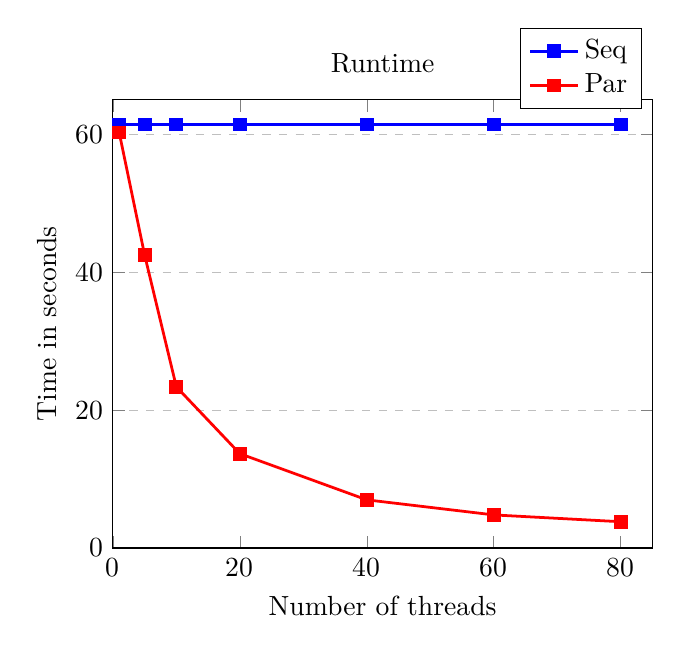
\begin{tikzpicture}
      \begin{axis}[
        title={Runtime},
        xlabel={Number of threads},
        ylabel={Time in seconds},
        ymin=0, ymax=65,
        xmin=0, xmax=85,
        ymajorgrids=true,
        grid style=dashed,
        legend style={anchor=south east}
        ]

        \addplot[color=blue,mark=square*,line width=1pt]
        coordinates {
          (1,  61.414685)
          (5, 61.414685)
          (10, 61.414685)
          (20, 61.414685)
          (40, 61.414685)
          (60, 61.414685)
          (80, 61.414685)
        };
        \addplot[color=red,mark=square*,line width=1pt]
        coordinates {
          (1, 60.241224)
          (5, 42.505744)
          (10, 23.375631)
          (20, 13.683191)
          (40, 6.987723)
          (60, 4.803215)
          (80, 3.813177)
        };
        \legend{Seq, Par}
      \end{axis}
    \end{tikzpicture}
  \end{minipage}\hfill
  \begin{minipage}[t]{.37\linewidth}
    \centering
    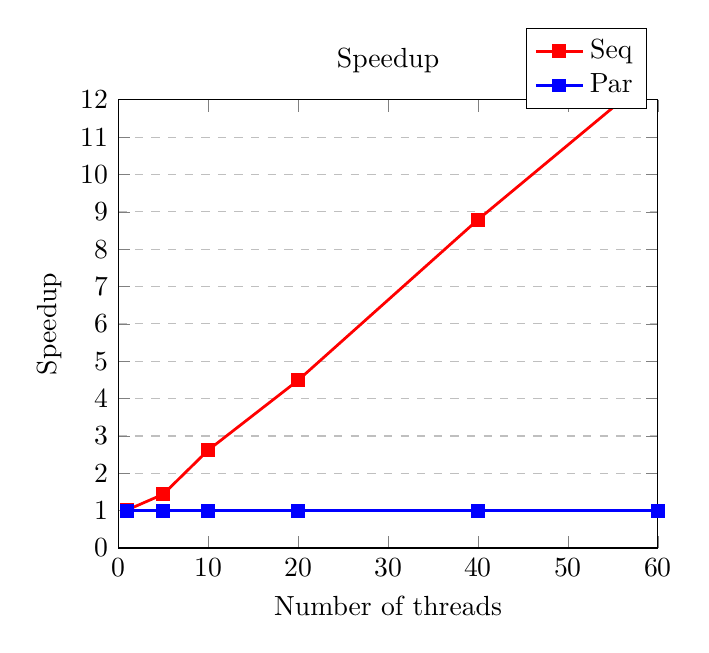
\begin{tikzpicture}
      \begin{axis}[
        title={Speedup},
        xlabel={Number of threads},
        ylabel={Speedup},
        xmin=0, xmax=60,
        ymin=0, ymax=12,
        ytick={0,1,...,14},
        ymajorgrids=true,
        grid style=dashed,
        legend style={anchor=south east}
        ]

        \addplot[color=red,mark=square*,line width=1pt]
        coordinates {
          (1, 1.02)
          (5, 1.44)
          (10, 2.62)
          (20, 4.49 )
          (40, 8.79)
          (60, 12.79)
          (80, 16.10)
        };
        \addplot[color=blue,mark=square*,line width=1pt]
        coordinates { (1, 1 ) (5, 1 ) (10, 1 ) (20, 1 ) (40, 1 ) (60, 1 ) (80, 1) };
        \legend{Seq, Par}
      \end{axis}
    \end{tikzpicture}
  \end{minipage}
  \caption{Plot for runtime and speedup}
\end{figure}

\clearpage

\section{Merge sort}
The results shown in the table come from sorting a list of 80000000 randomly selected integers. The relatively quick change in runtime for number of threads stem from the fact that these tests were run locally.
\begin{table}[ht]
  \centerfloat
  \begin{tabulary}{.4\linewidth}{ rrrr }
    \toprule
    Num threads & Runtime    & Speedup \\
    \midrule
    1           & 11.305429s  & 1.00 \\
    5           & 4.994405s  & 2.26 \\
    10          & 3.578300s  & 3.15  \\
    20          & 4.131745s  & 2.73  \\
    \bottomrule
  \end{tabulary}
  \caption{Merge sort}\label{table:mandel}
\end{table}

\begin{figure}[ht]
  \centerfloat
  \begin{minipage}[t]{.4\linewidth}
    \centering
    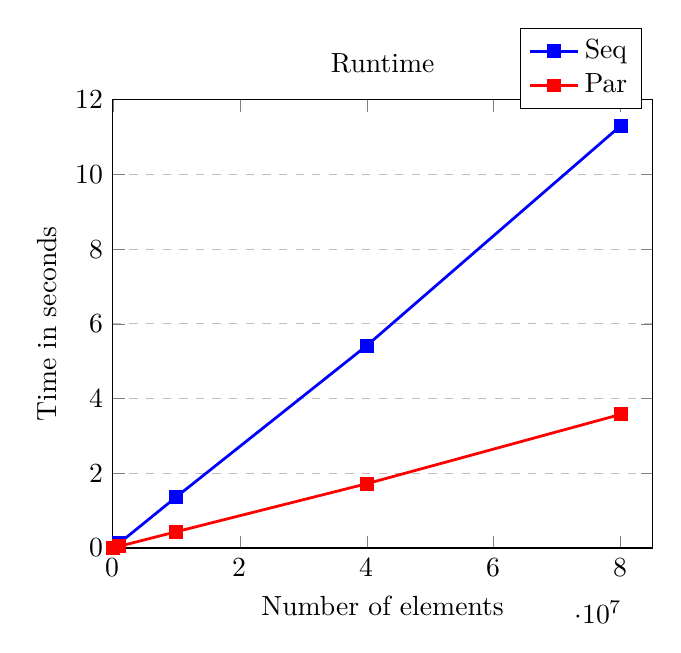
\begin{tikzpicture}
      \begin{axis}[
        title={Runtime},
        xlabel={Number of elements},
        ylabel={Time in seconds},
        ymin=0, ymax=12,
        xmin=0, xmax=85000000,
        ymajorgrids=true,
        grid style=dashed,
        legend style={anchor=south east}
        ]

        \addplot[color=blue,mark=square*,line width=1pt]
        coordinates {
          (10000,  0.000910)
          (100000, 0.009904)
          (1000000, 0.129268)
          (10000000, 1.369713)
          (40000000, 5.419183)
          (80000000, 11.305429)
        };
        \addplot[color=red,mark=square*,line width=1pt]
        coordinates {
          (10000,  0.009759)
          (100000, 0.016566)
          (1000000, 0.047348)
          (10000000, 0.437084)
          (40000000, 1.722421)
          (80000000, 3.578300)
        };
        \legend{Seq, Par}
      \end{axis}
    \end{tikzpicture}
  \end{minipage}\hfill
  \begin{minipage}[t]{.37\linewidth}
    \centering
    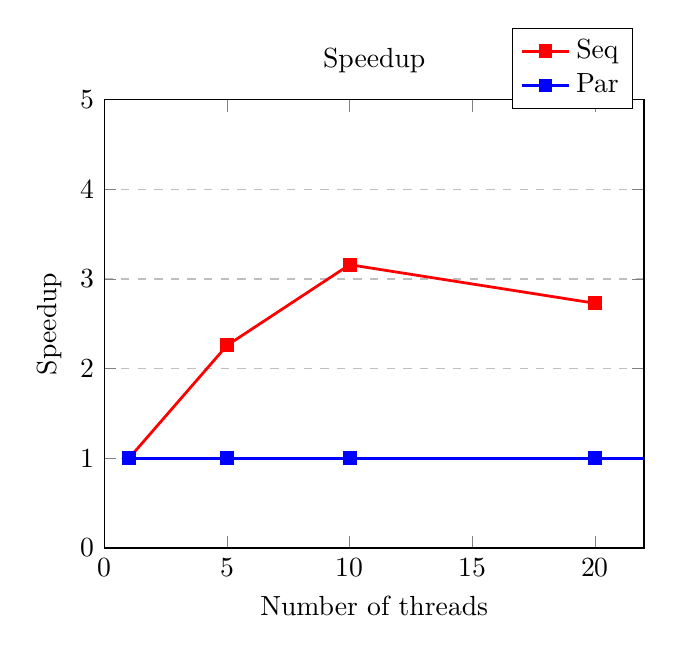
\begin{tikzpicture}
      \begin{axis}[
        title={Speedup},
        xlabel={Number of threads},
        ylabel={Speedup},
        xmin=0, xmax=22,
        ymin=0, ymax=5,
        ytick={0,1,...,14},
        ymajorgrids=true,
        grid style=dashed,
        legend style={anchor=south east}
        ]

        \addplot[color=red,mark=square*,line width=1pt]
        coordinates {
          (1, 1.00)
          (5, 2.26)
          (10, 3.16)
          (20, 2.73 )
        };
        \addplot[color=blue,mark=square*,line width=1pt]
        coordinates { (1, 1 ) (5, 1 ) (10, 1 ) (20, 1 ) (40, 1 ) (60, 1 ) (80, 1) };
        \legend{Seq, Par}
      \end{axis}
    \end{tikzpicture}
  \end{minipage}
  \caption{Plot for runtime and speedup}
\end{figure}

\clearpage

\chapter{Conclusion} % (fold)
\label{cha:Conclusion}

\section{Mandelbrot} % (fold)
\label{sec:Mandelbrot}

As we can see from the runtime and speedup of the mandelbrot problem it is what 
I think you can call ``embarrassingly parallelizable''. The speed increase is nearly
linear. This makes sense for this particular implementation as the whole program is
essentially two for loops where there is no need to keep track of data per thread. 

Compared to the algorithm for mandatory 2 and 1 where the parallel implementation needed
guards and calculating prefix sums and so on, this is just a simple loop and add 
data to an array. We initially thought that this problem would be more complex, but 
as it turns out it wasn't. 

Because it was so simple we planned on attempting a SIMD variant of the program
to see if pipelining and such would yield a speedup, but our lack of knowledge 
on both C/C++ and SIMD made this a pipe dream. We suspect it would speed everything
up a bit again, as being able to do multiplication across multiple rows or columns
should logically yield a speedup.

\section{Merge sort}
Merge sort has a runtime of O(nlog n). The theoretical speedup for the parallel algorithm is p, the numbers of threads, when n = p. Then, in every step of the iteration, we hand out all chunks to their own thread, saving O(log n) runtime over O(n) iterations. Therefore we expect the runtime of the parallel program to be O(nlog n) / O(log n) = O(n). Except for lesser number of elements, where the startup costs outweigh the time saved, and is therefore slower than the sequential program.

In none of the tests the results are as good as in theory, but this might be hardware specific, because as of now we have yet to test the program on brake.
% chapter Conclusion (end)
\end{document}
%%% Local Variables:
%%% mode: latex
%%% TeX-master: t
%%% End:
